% !TeX root = ../main.tex

\chapter{Results}\label{results}
We are going to analyze the estimation results of ATT with the delicately determined anticipation parameter (see \nameref{sec:anticipation}) and the assumption of unconditional PTA.
To understand the magnitudes of the estimated effects, we will naively employ the mean outcome of the control group in September 2013 as the baseline for the context of residential shifts, while for smartphone adoption, the baseline will be that of October 2013.
The confidence interval is constructed based on the 95\% significance level. We first analyze heterogeneous treatment effects across time periods.
Specifically, we will approach with a hierarchical manner starting from the discussion of static versus time-variant treatment effects.
The static treatment effect means the outcome is persistently shifted without fading back to the baseline level.
In such situation, attribution includes upward or downward shift.
For the time-variant one, we can characterize it to be either transient or smoothly decaying.
A transient treatment effect over time represents an effect that instantly bounces back and forth to the baseline, while smoothly decaying is the other case, where the effect gradually fades away.
Then, we can discuss the heterogeneous effect across treatment-timing groups by inspecting whether only few groups exhibit distinct patterns.

\clearpage\newpage
\section{Residential Shifts}\label{main_res_residential_shift}
\begin{figure}[h!]
\centering
\caption{Aggregated Event Study of Residential Shifts}
\vspace{0.1cm}

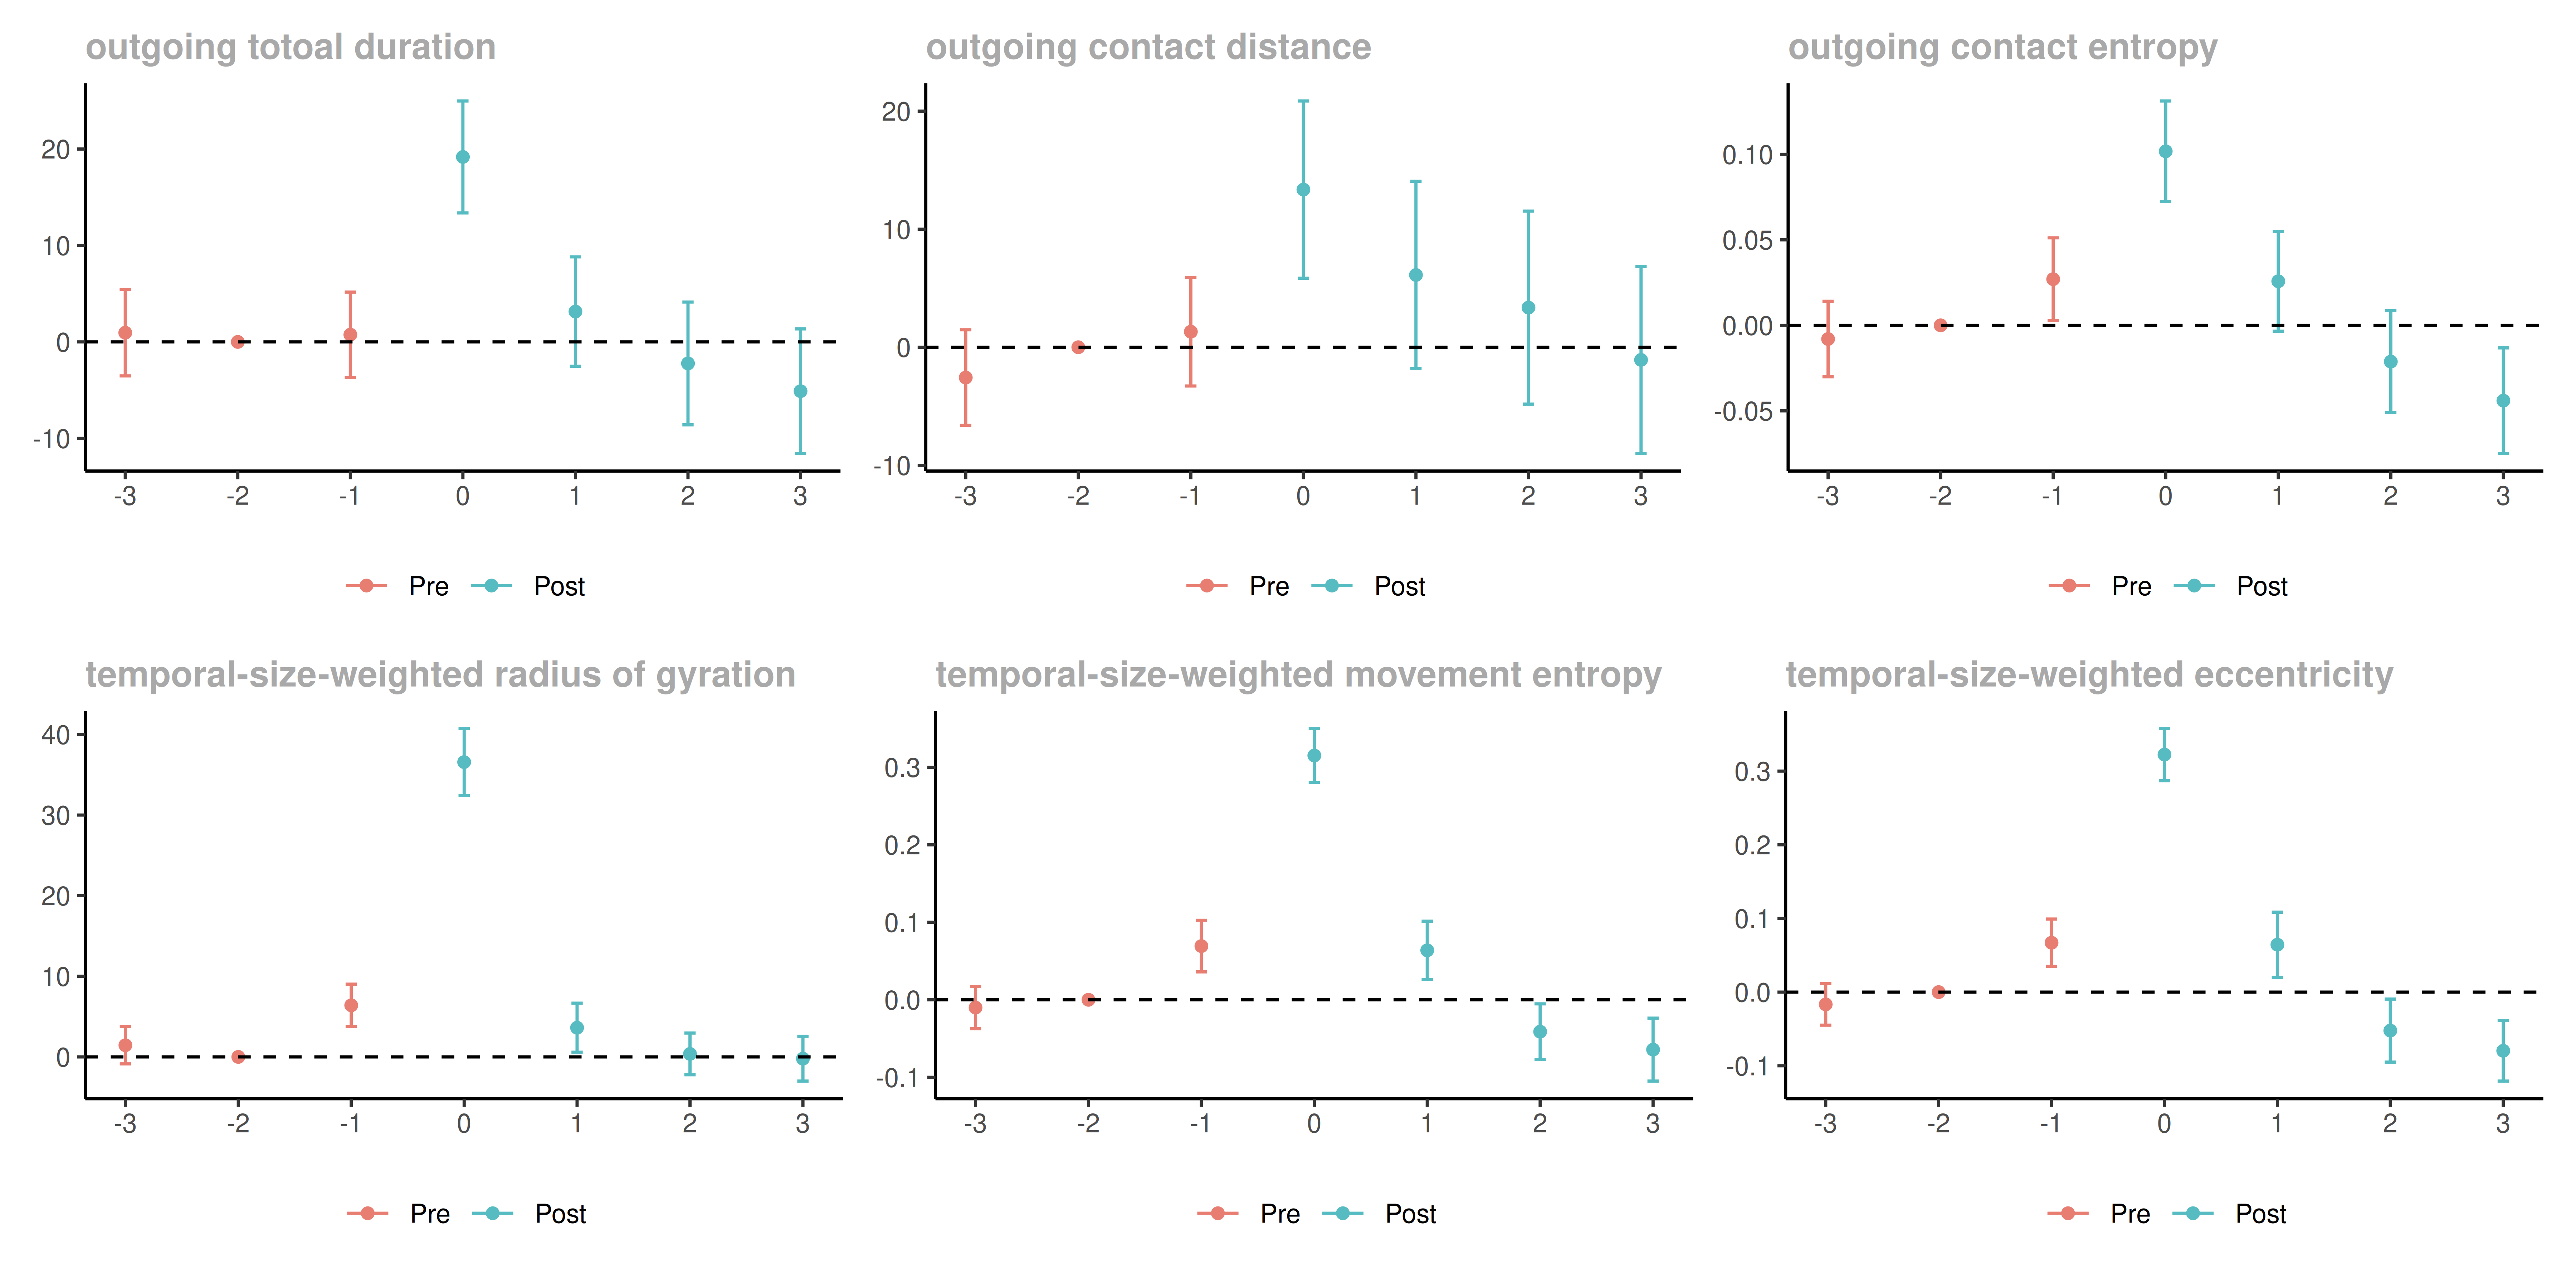
\includegraphics[scale=0.49]{figures/csdid/residential_shift.png}

% \caption*{Notes:}
\label{fig:event_study_residential_shift}
\end{figure}

At the very first glance, we can see that the residential shift brings about time-variant effects on both mobile communication network (upper panel) and mobility features (lower panel), and effects fall back to or approach to the baseline level one month after relocations begin.

For the mobile communication behavior, anticipation for residential relocation is limited and observable only in outgoing contact entropy.
The pre-treatment shift in outgoing contact entropy might be result from notifying forthcoming relocation with friends that are less frequently contacted.
However, from Figure~\ref{fig:attgt_residential_shift_mobile_communication_network}, we can see that this phenomenon only emerges in the treated units who migrate in February 2014 (group 7).

Intuitively, residential relocations expose mobile phone users to unfamiliar environments, resulting in a temporary surge in total call duration during the month of relocation.
Relative to the baseline mean of 89.7 minutes, migrants experience a 19 minute (21\%) increase in outgoing call duration, and a 13 km (189\%) increase in outgoing contact distance relative to the baseline mean of 6.9 km as they seek to connect with geographically distant social connections.
Moreover, during this same period, migrants engage in more diversified social interactions, with entropy increasing by 0.10 units (a 17\% increase from the baseline of 0.60), likely due to the formation of new social connections at the destination or contact with those with whom they engaged less frequently prior to the relocation
Nevertheless, following the completion of relocation, migrants tend to spend less time on mobile communication with less diversified interactions. By the third month post-relocation, total call duration decreases by 5.1 minutes (a 6\% reduction from the 89.7-minute baseline) and contact entropy falls by 0.04 units (a 7\% decrease from the baseline of 0.60), indicating a return toward more concentrated communication patterns.


\begin{figure}[h!]
\centering
\caption{Contact Ratio of Pre-Treatment Friends in Post-Treatment Periods}

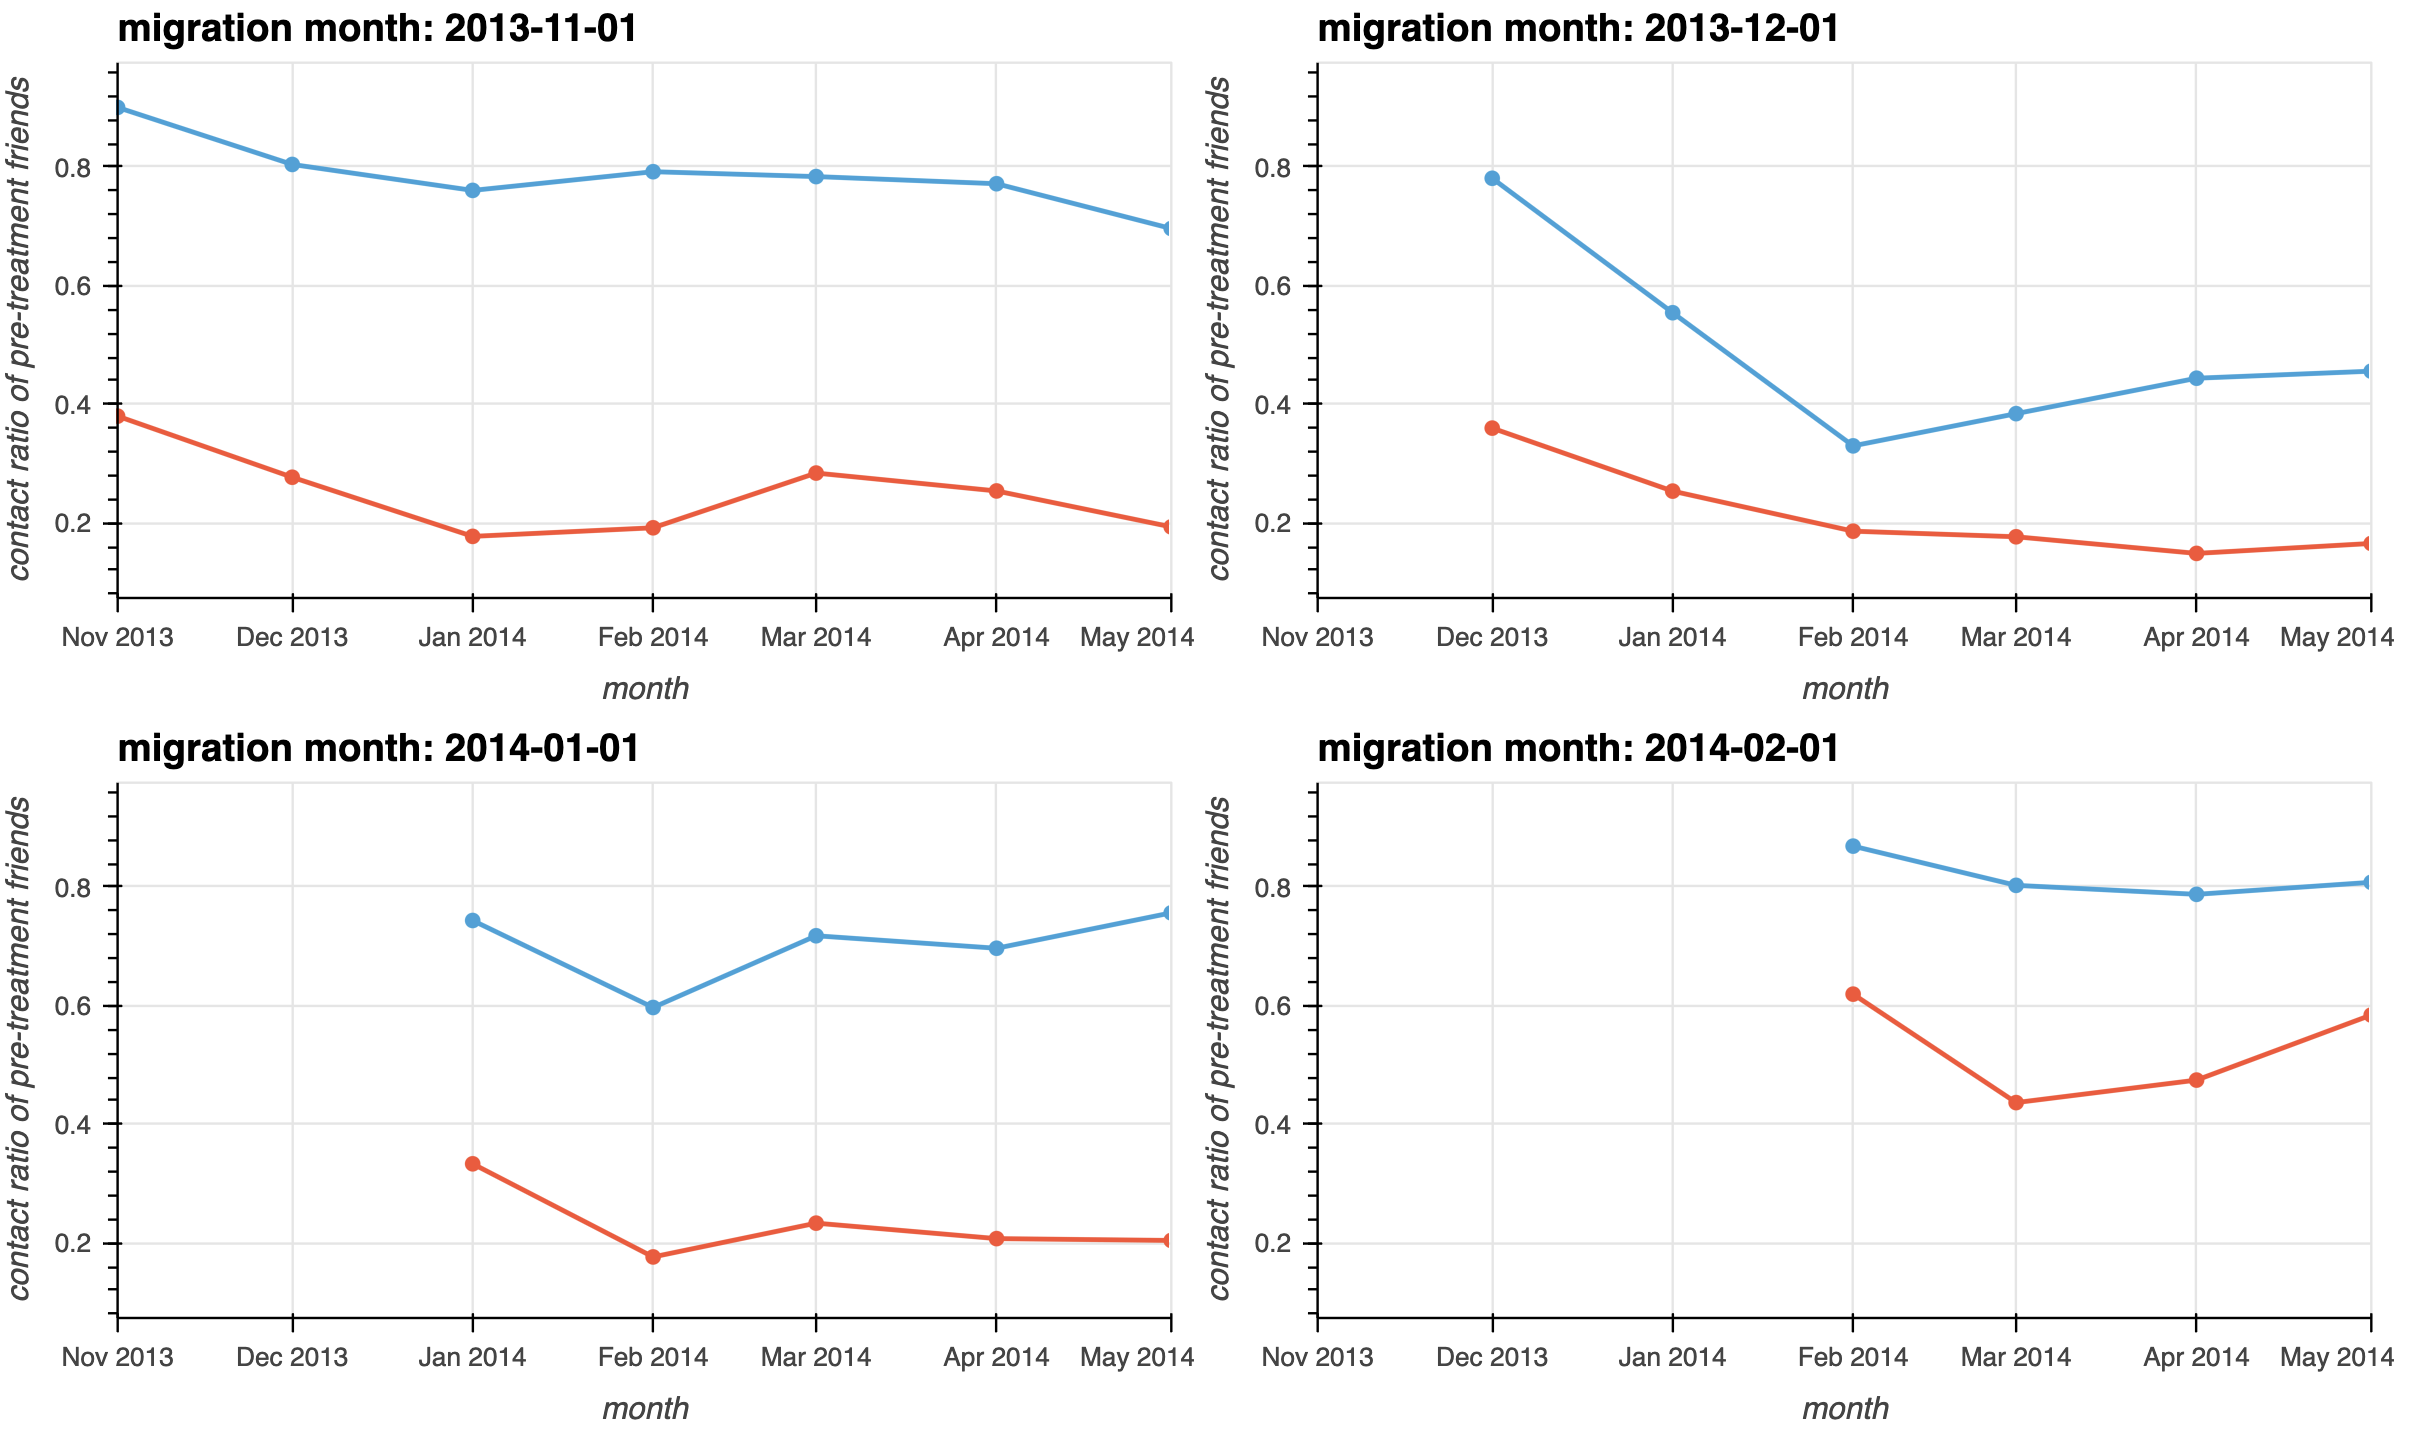
\includegraphics[scale=0.35]{figures/contact_ratio_of_pretreatment_friends.png}

\caption*{Notes: The blue line is the contact ratio of pre-treatment friends while the red line additionally require those in the same origin prefecture.}
\label{fig:contact_ratio_old_friends}
\end{figure}


In Figure \ref{fig:contact_ratio_old_friends}, we analyze the composition of migrants' contacts in post relocation periods.
We define a new variable called contact ratio, and the contact ratio of a user in a given month measures the proportion of the users' call duration with friends with whom they are already connected versus all friends contacted in the corresponding month.
In the above plot, we present the monthly contact ratio series obtained by averaging across all users in each given month.
We also separately plot the contact ratios for migrants who relocate in different months though they seem to behave very similarly.

We can confirm that, in the early periods of post-migration, migrants tend to connect with those old friends with whom are already connected prior to the migration events.
Typically, in the same months of changing residential places, around 80\% of contacts are pre-treatment friends, but they are not necessarily in the same prefectures from which migrants come.
Specifically, roughly 40\% of these pre-treatment friends reside in the migrants' origin prefecture.
These facts support the hypothesis that the sudden surge in mobile communication during the period of migration is due to connections with existing friendships.
Moreover, the drastic increase in contact distance also suggests that migrants move away from their friends rather than toward them.

For mobility patterns, the evidence of anticipation behavior is even more solidified, with moderate upward shift.
The spatial coverage of movement activity measured through the metric of radius of gyration substantially increases contemporaneously with the completion of residential relocation, expanding by 36.6 km (a 412\% increase from the 8.9 km baseline) while the effect quickly fades back in the following months. This substantial increase includes the component of traveling distance between the origin and destination locations during the relocation process.
Movement entropy and eccentricity evolve in an extreme pattern where migrants instantly transit from highly unpredictable spatial appearances with spatial stretching along a fixed direction to predictable patterns with roughly circular spatial distribution.
This is characterized by a dramatic shift from 0.32 above the entropy baseline of 0.67 (a 47\% increase) and 0.32 above the eccentricity baseline of 0.82 (a 39\% increase) during relocation month, to -0.06 (9\% below baseline) and -0.08 (10\% below baseline) respectively by the third month post-relocation. The intuition is that when moving to a new environment, a migrant might be actively exploring but have limited knowledge, resulting in exploration along a fixed axis. As time passes, exploration patterns settle down, and they mainly visit a few places located in various directions, creating a more balanced and predictable spatial distribution.

% In conclusion, residential shifts produce distinct anticipation effects between communication and mobility domains, with mobility patterns showing more pronounced responses than communication behaviors.
% Both groups of features seem to be continuously evolving to negative states. To better understand the evolving paths of various features across treatment-timing groups, please refer to \nameref{complete_group_time_att_dynamics}.

% \clearpage\newpage
\section{Smartphone Adoption}
\begin{figure}[h!]
\centering
\caption{Aggregate Event Study of Smartphone Adoption}
\vspace{0.1cm}

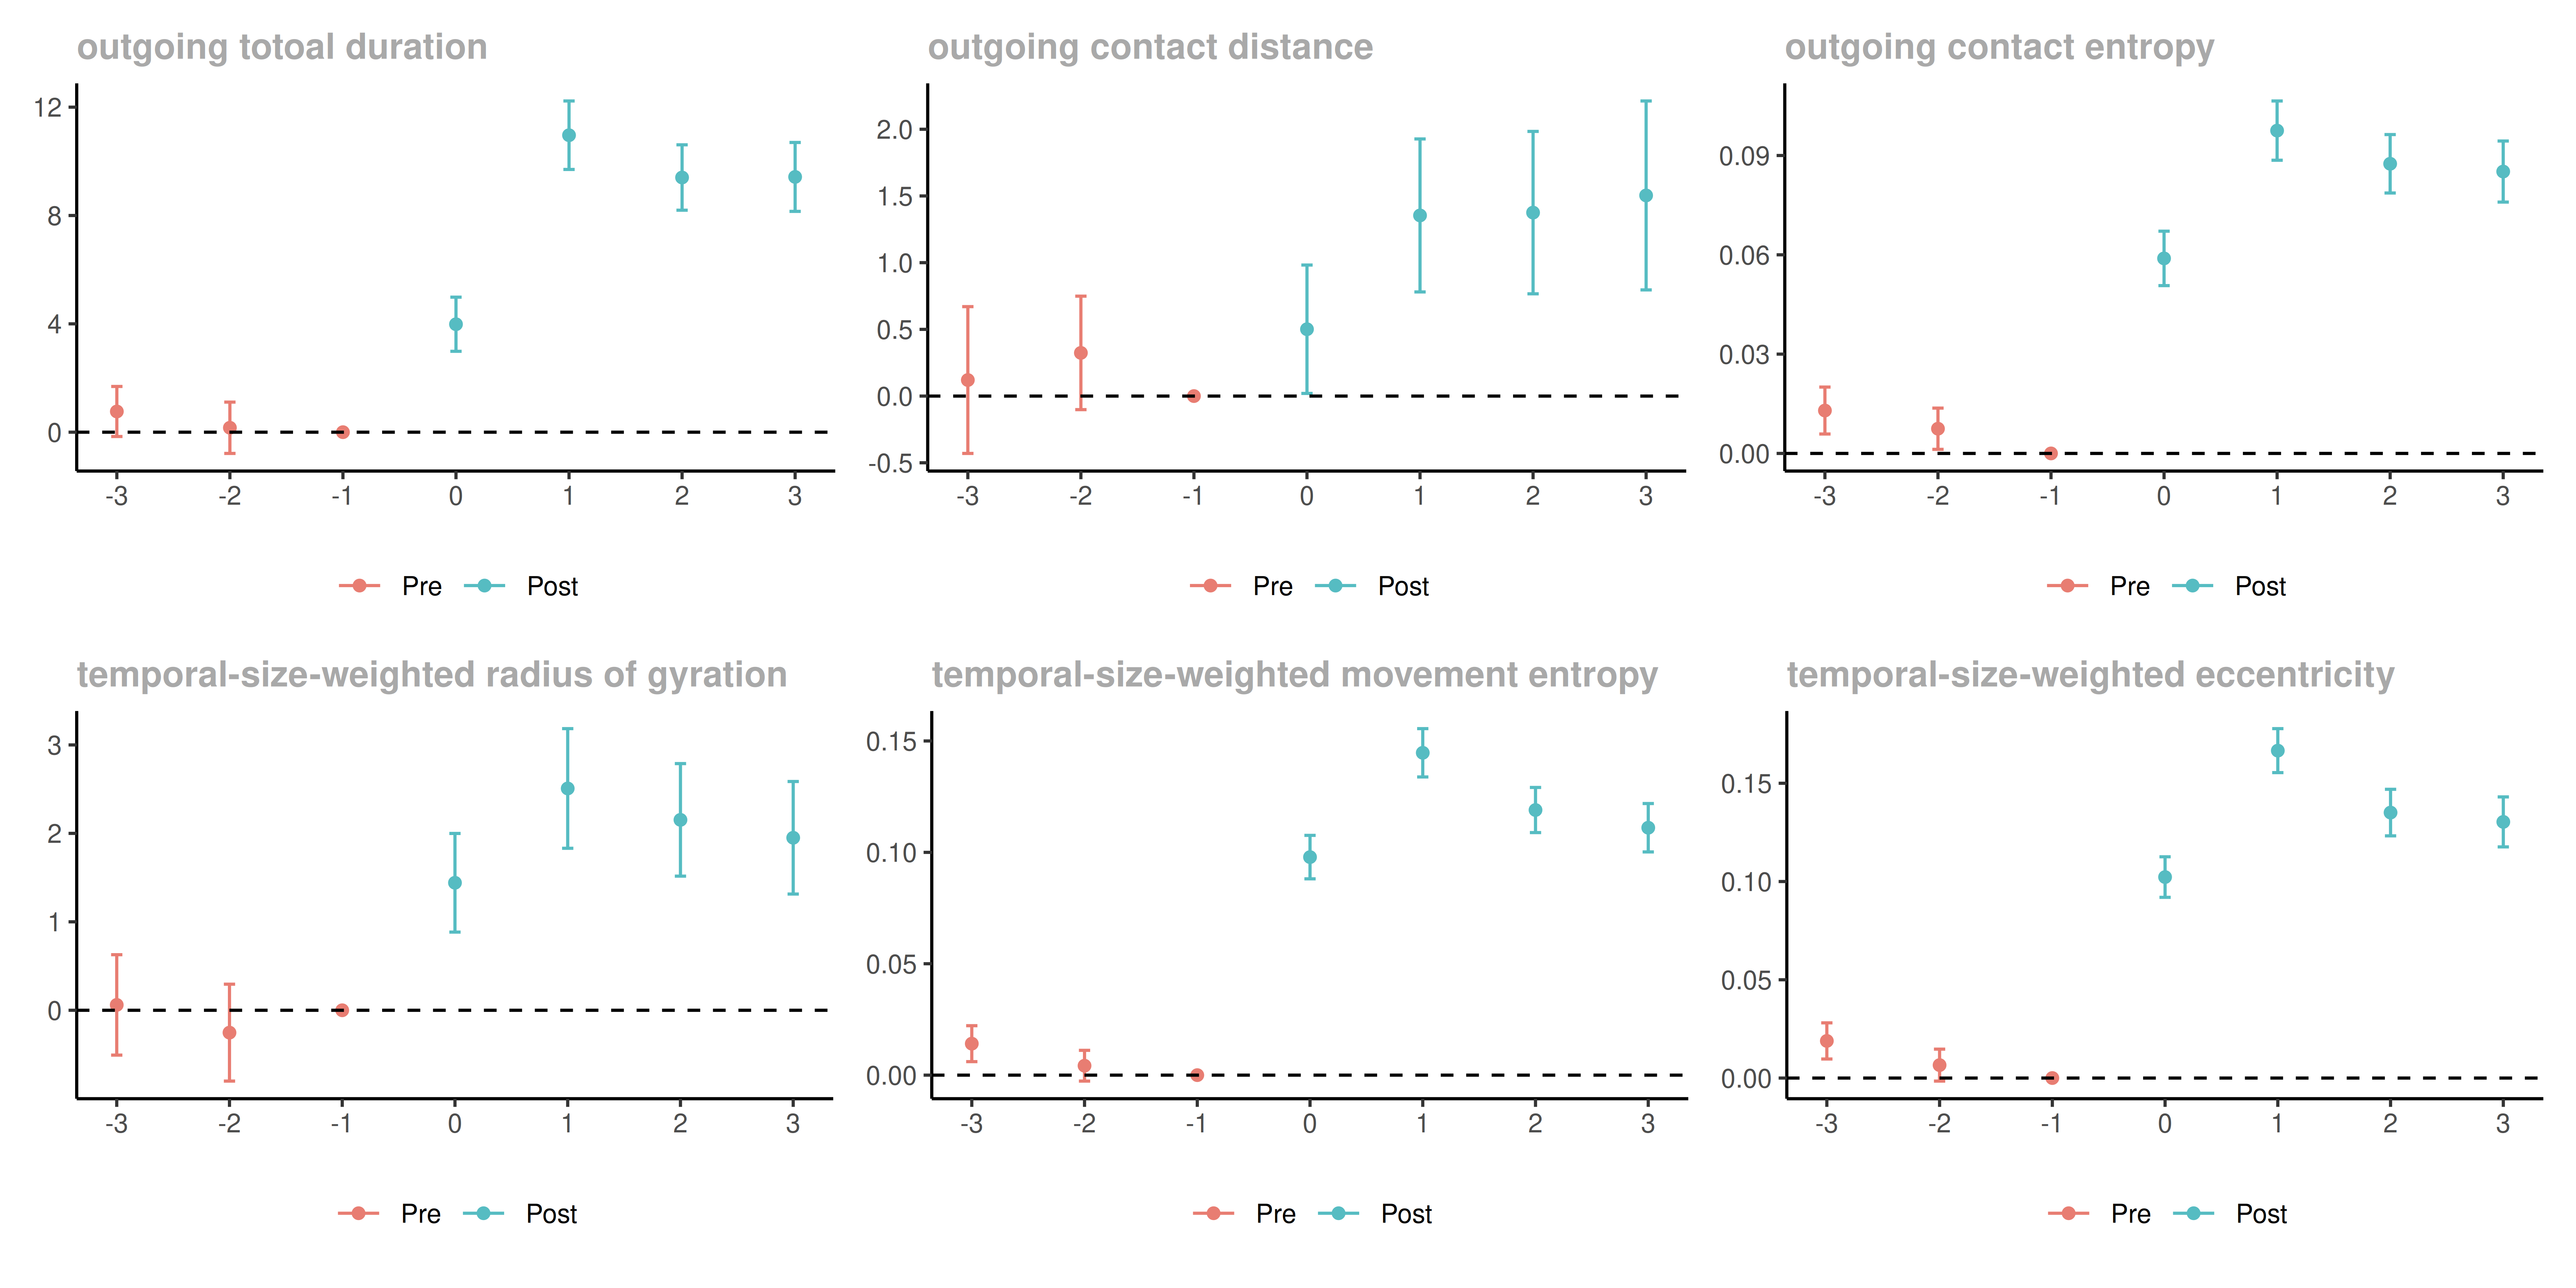
\includegraphics[scale=0.49]{figures/csdid/smartphone_adoption.png}

% \caption*{Notes:}
\label{fig:event_study_smartphone_adoption}
\end{figure}

Unlike the residential shift, we expect no anticipation for smartphone adoption.
We clearly see that the effects are nearly static over time and the shifts are positive, but the magnitude is relatively small compared to the residential shift.
By inspecting ATT dynamics across different groups demonstrated in both Figure \ref{fig:attgt_smartphone_adoption_mobile_communication_network} and \ref{fig:attgt_smartphone_adoption_mobility}, we can confirm that there is no heterogeneous effect across groups.

Relative to the non-smartphone users' baseline in October 2013, smartphone adoption leads to immediate behavioral changes.
The most notable influence is the increase in radius of gyration by 1.4 km (a 21\% increase from the 6.8 km baseline).
There are also modest shifts in movement entropy (0.10 units, 16\% increase from the 0.62 baseline) and eccentricity (0.10 units, 13\% increase from the 0.78 baseline), along with smaller increases in contact entropy of 0.06 units (10\% increase from the 0.57 baseline) and call duration of 4.0 minutes (9\% increase from the 44.8 minutes baseline).

The shifts in movement entropy and eccentricity likely reflect the integration of geographical technologies, such as online maps, facilitating exploration of unfamiliar places.
Interestingly, this pattern is identical to that observed during residential relocations, where individuals moving to new environments exhibit increased movement entropy (exploring behavior) coupled with increased eccentricity (fixed directional preference).
This finding additionally confirms the systematic "exploring pattern of individuals" where users do not tend to explore randomly but rather follow structured exploration along preferred directions, suggesting that smartphone adoption triggers similar exploratory behaviors as physical relocation to unfamiliar territories.

It seems counterintuitive that after upgrading to smartphone devices, users increase their call duration as they might have better access to the internet and switch to using mobile communication apps like WeChat.
Our explanation is that our examination of effect dynamics is on a monthly basis, which is short-term, and these users originally used non-smartphones, which might suggest that they don't have a strong preference for the internet and tend to utilize phone calls to contact their friends.
Therefore, after upgrading to smartphones, in the short run, they might still mainly rely on phone calls rather than the internet to interact with their friends.
Besides, we believe that mobile infrastructure was not well implemented back in 2013 when 4G technology was not widely spread.
Therefore, phone calls still served as a major tunnel for remote social interactions.
